\documentclass{standalone}
\usepackage{tikz}
\usetikzlibrary{patterns, positioning}


\begin{document}
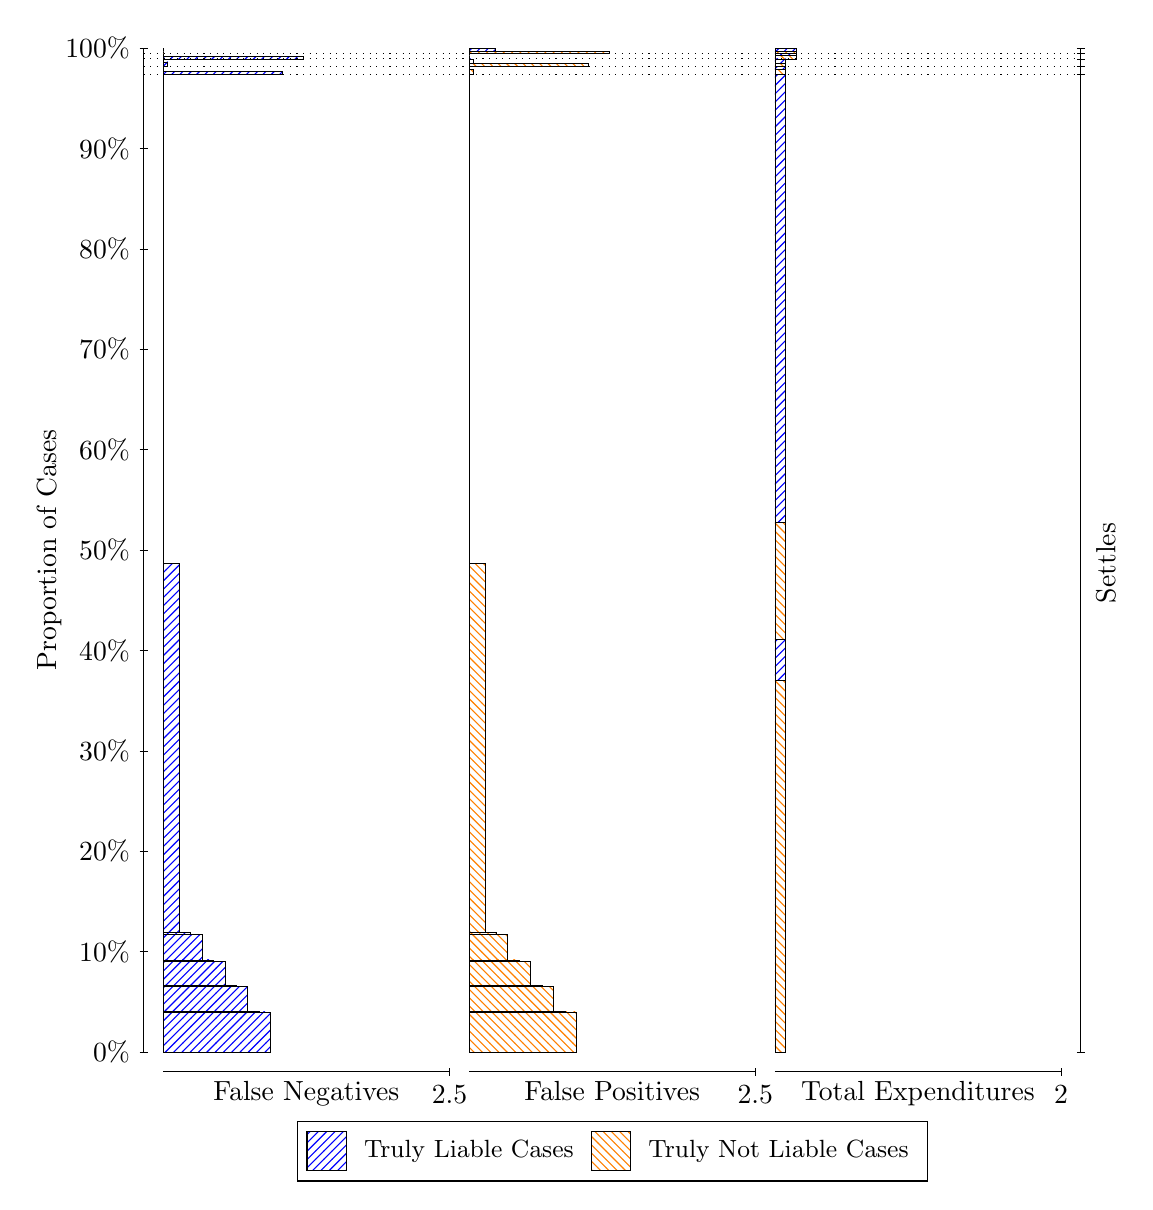
\begin{tikzpicture}
\draw[black, very thin] (1.5,1.75) -- (1.5,14.5);
\node[rotate=90, text=black, anchor=center] at (0.3, 8.125) {Proportion of Cases};
\draw[black, very thin] (1.45,1.75) -- (1.55,1.75);
\node[text=black, anchor=east] at (1.45, 1.75) {0\%};
\draw[black, very thin] (1.45,3.025) -- (1.55,3.025);
\node[text=black, anchor=east] at (1.45, 3.025) {10\%};
\draw[black, very thin] (1.45,4.3) -- (1.55,4.3);
\node[text=black, anchor=east] at (1.45, 4.3) {20\%};
\draw[black, very thin] (1.45,5.575) -- (1.55,5.575);
\node[text=black, anchor=east] at (1.45, 5.575) {30\%};
\draw[black, very thin] (1.45,6.85) -- (1.55,6.85);
\node[text=black, anchor=east] at (1.45, 6.85) {40\%};
\draw[black, very thin] (1.45,8.125) -- (1.55,8.125);
\node[text=black, anchor=east] at (1.45, 8.125) {50\%};
\draw[black, very thin] (1.45,9.4) -- (1.55,9.4);
\node[text=black, anchor=east] at (1.45, 9.4) {60\%};
\draw[black, very thin] (1.45,10.675) -- (1.55,10.675);
\node[text=black, anchor=east] at (1.45, 10.675) {70\%};
\draw[black, very thin] (1.45,11.95) -- (1.55,11.95);
\node[text=black, anchor=east] at (1.45, 11.95) {80\%};
\draw[black, very thin] (1.45,13.225) -- (1.55,13.225);
\node[text=black, anchor=east] at (1.45, 13.225) {90\%};
\draw[black, very thin] (1.45,14.5) -- (1.55,14.5);
\node[text=black, anchor=east] at (1.45, 14.5) {100\%};

\draw[black, very thin] (13.4,1.75) -- (13.4,14.5);
\draw[black, very thin] (13.35,1.75) -- (13.45,1.75);
\node[anchor=west] at (13.35, 1.75) {};
\draw[black, very thin] (13.35,14.169) -- (13.45,14.169);
\node[anchor=west] at (13.35, 14.169) {};
\draw[black, very thin] (13.35,14.265) -- (13.45,14.265);
\node[anchor=west] at (13.35, 14.265) {};
\draw[black, very thin] (13.35,14.362) -- (13.45,14.362);
\node[anchor=west] at (13.35, 14.362) {};
\draw[black, very thin] (13.35,14.431) -- (13.45,14.431);
\node[anchor=west] at (13.35, 14.431) {};
\draw[black, very thin] (13.35,14.5) -- (13.45,14.5);
\node[anchor=west] at (13.35, 14.5) {};

\draw[black, very thin, pattern color=blue, pattern=north east lines] (1.75,1.75) rectangle (3.1125,2.2594);
\draw[black, very thin, pattern color=blue, pattern=north east lines] (1.75,2.2594) rectangle (2.9672,2.2698);
\draw[black, very thin, pattern color=blue, pattern=north east lines] (1.75,2.2698) rectangle (2.8218,2.583);
\draw[black, very thin, pattern color=blue, pattern=north east lines] (1.75,2.583) rectangle (2.6765,2.5934);
\draw[black, very thin, pattern color=blue, pattern=north east lines] (1.75,2.5934) rectangle (2.5312,2.8968);
\draw[black, very thin, pattern color=blue, pattern=north east lines] (1.75,2.8968) rectangle (2.3858,2.9186);
\draw[black, very thin, pattern color=blue, pattern=north east lines] (1.75,2.9186) rectangle (2.2405,3.2433);
\draw[black, very thin, pattern color=blue, pattern=north east lines] (1.75,3.2433) rectangle (2.0952,3.2652);
\draw[black, very thin, pattern color=blue, pattern=north east lines] (1.75,3.2652) rectangle (1.9498,7.9594);
\draw[black, very thin, pattern color=orange, pattern=north west lines] (1.75,7.9594) rectangle (1.75,14.169);
\draw[black, very thin, pattern color=blue, pattern=north east lines] (1.75,14.169) rectangle (3.2578,14.207);
\draw[black, very thin, pattern color=orange, pattern=north west lines] (1.75,14.207) rectangle (1.75,14.265);
\draw[black, very thin, pattern color=blue, pattern=north east lines] (1.75,14.265) rectangle (1.8045,14.324);
\draw[black, very thin, pattern color=orange, pattern=north west lines] (1.75,14.324) rectangle (1.75,14.362);
\draw[black, very thin, pattern color=blue, pattern=north east lines] (1.75,14.362) rectangle (3.5303,14.389);
\draw[black, very thin, pattern color=orange, pattern=north west lines] (1.75,14.389) rectangle (1.75,14.431);
\draw[black, very thin, pattern color=orange, pattern=north west lines] (1.75,14.431) rectangle (1.75,14.458);
\draw[black, very thin, pattern color=blue, pattern=north east lines] (1.75,14.458) rectangle (1.75,14.5);
\draw[black, very thin, pattern color=orange, pattern=north west lines] (5.6333,1.75) rectangle (6.9958,2.2594);
\draw[black, very thin, pattern color=orange, pattern=north west lines] (5.6333,2.2594) rectangle (6.8505,2.2698);
\draw[black, very thin, pattern color=orange, pattern=north west lines] (5.6333,2.2698) rectangle (6.7052,2.583);
\draw[black, very thin, pattern color=orange, pattern=north west lines] (5.6333,2.583) rectangle (6.5598,2.5934);
\draw[black, very thin, pattern color=orange, pattern=north west lines] (5.6333,2.5934) rectangle (6.4145,2.8968);
\draw[black, very thin, pattern color=orange, pattern=north west lines] (5.6333,2.8968) rectangle (6.2692,2.9186);
\draw[black, very thin, pattern color=orange, pattern=north west lines] (5.6333,2.9186) rectangle (6.1238,3.2433);
\draw[black, very thin, pattern color=orange, pattern=north west lines] (5.6333,3.2433) rectangle (5.9785,3.2652);
\draw[black, very thin, pattern color=orange, pattern=north west lines] (5.6333,3.2652) rectangle (5.8332,7.9594);
\draw[black, very thin, pattern color=blue, pattern=north east lines] (5.6333,7.9594) rectangle (5.6333,14.169);
\draw[black, very thin, pattern color=orange, pattern=north west lines] (5.6333,14.169) rectangle (5.6878,14.227);
\draw[black, very thin, pattern color=blue, pattern=north east lines] (5.6333,14.227) rectangle (5.6333,14.265);
\draw[black, very thin, pattern color=orange, pattern=north west lines] (5.6333,14.265) rectangle (7.1412,14.303);
\draw[black, very thin, pattern color=blue, pattern=north east lines] (5.6333,14.303) rectangle (5.6878,14.362);
\draw[black, very thin, pattern color=orange, pattern=north west lines] (5.6333,14.362) rectangle (5.6333,14.404);
\draw[black, very thin, pattern color=blue, pattern=north east lines] (5.6333,14.404) rectangle (5.6333,14.431);
\draw[black, very thin, pattern color=orange, pattern=north west lines] (5.6333,14.431) rectangle (7.4137,14.458);
\draw[black, very thin, pattern color=blue, pattern=north east lines] (5.6333,14.458) rectangle (5.9603,14.5);
\draw[black, very thin, pattern color=orange, pattern=north west lines] (9.5167,1.75) rectangle (9.6529,6.4661);
\draw[black, very thin, pattern color=blue, pattern=north east lines] (9.5167,6.4661) rectangle (9.6529,6.9859);
\draw[black, very thin, pattern color=orange, pattern=north west lines] (9.5167,6.9859) rectangle (9.6529,8.4792);
\draw[black, very thin, pattern color=blue, pattern=north east lines] (9.5167,8.4792) rectangle (9.6529,14.169);
\draw[black, very thin, pattern color=orange, pattern=north west lines] (9.5167,14.169) rectangle (9.6529,14.227);
\draw[black, very thin, pattern color=blue, pattern=north east lines] (9.5167,14.227) rectangle (9.6529,14.265);
\draw[black, very thin, pattern color=orange, pattern=north west lines] (9.5167,14.265) rectangle (9.6529,14.303);
\draw[black, very thin, pattern color=blue, pattern=north east lines] (9.5167,14.303) rectangle (9.6529,14.362);
\draw[black, very thin, pattern color=orange, pattern=north west lines] (9.5167,14.362) rectangle (9.7892,14.404);
\draw[black, very thin, pattern color=blue, pattern=north east lines] (9.5167,14.404) rectangle (9.7892,14.431);
\draw[black, very thin, pattern color=orange, pattern=north west lines] (9.5167,14.431) rectangle (9.7892,14.458);
\draw[black, very thin, pattern color=blue, pattern=north east lines] (9.5167,14.458) rectangle (9.7892,14.5);
\draw[black, dotted] (1.5,14.169) -- (13.4,14.169);
\draw[black, dotted] (1.5,14.265) -- (13.4,14.265);
\draw[black, dotted] (1.5,14.362) -- (13.4,14.362);
\draw[black, dotted] (1.5,14.431) -- (13.4,14.431);
\draw[black, very thin] (1.75,1.5) -- (5.3833,1.5);
\node[text=black, anchor=north] at (3.5667, 1.5) {False Negatives};
\draw[black, very thin] (5.3833,1.45) -- (5.3833,1.55);
\node[text=black, anchor=north] at (5.3833, 1.45) {2.5};

\draw[black, very thin] (5.6333,1.5) -- (9.2667,1.5);
\node[text=black, anchor=north] at (7.45, 1.5) {False Positives};
\draw[black, very thin] (9.2667,1.45) -- (9.2667,1.55);
\node[text=black, anchor=north] at (9.2667, 1.45) {2.5};

\draw[black, very thin] (9.5167,1.5) -- (13.15,1.5);
\node[text=black, anchor=north] at (11.333, 1.5) {Total Expenditures};
\draw[black, very thin] (13.15,1.45) -- (13.15,1.55);
\node[text=black, anchor=north] at (13.15, 1.45) {2};

\node[text=black, centered, rotate=90] at (13.72, 7.9594) {Settles};





\draw (7.449999999999999,1.5) node[draw=none] (baseCoordinate) {};
\begin{scope}[align=center]
        \matrix[scale=0.5, draw=black, below=0.5cm of baseCoordinate, nodes={draw}, column sep=0.1cm]{
            \node[rectangle, draw, minimum width=0.5cm, minimum height=0.5cm, pattern color=blue, pattern=north east lines] {}; &
            \node[draw=none, font=\small, text=black] (B) {Truly Liable Cases}; &
            \node[rectangle, draw, minimum width=0.5cm, minimum height=0.5cm, pattern color=orange, pattern=north west lines] {}; &
            \node[draw=none, font=\small, text=black] (B) {Truly Not Liable Cases}; \\
            };
\end{scope}

\end{tikzpicture}
\end{document}